\documentclass{article}
\usepackage[utf8]{inputenc}
\usepackage[brazilian]{babel}
\usepackage{geometry}
\geometry{a4paper, total={150mm,240mm}, top=25mm}
\usepackage{graphicx}
\usepackage{titling}
\usepackage{float}
\usepackage{natbib}
\usepackage{setspace}
\onehalfspacing

\title{Trabalho 1 - Fecho Convexo}
\author{Kleyton da Costa (2312730)}
\date{\today}
 
\usepackage{fancyhdr}
\fancypagestyle{plain}{%  the preset of fancyhdr 
    \fancyhf{} % clear all header and footer fields
    \fancyfoot[R]{
\includegraphics[width=3cm]{di.png}}
    \fancyfoot[L]{\today}
    \fancyhead[L]{Geometria Computacional}
    \fancyhead[R]{\theauthor}
}
\makeatletter
\def\@maketitle{%
  \newpage
  \null
  \vskip 1em%
  \begin{center}%
  \let \footnote \thanks
    {\LARGE \@title \par}%
    \vskip 1em%
    %{\large \@date}%
  \end{center}%
  \par
  \vskip 1em}
\makeatother

\begin{document}

\maketitle

\noindent\begin{tabular}{@{}ll}
    Aluno & \theauthor \\
    Professor &  Waldemar Celes (DI/PUC-Rio)
\end{tabular}

\section{Motivação}

Este trabalho tem como objetivo descrever a aplicação de um algoritmo para a determinação do fecho convexo 2D para uma nuvem de pontos. Os experimentos levaram em consideração o algoritmo Jarvis March (ou \textit{Gift Wrapping}).

\section{Metodologia}

Um fecho convexo pode ser definido como o conjunto de todas as combinações convexas para um determinado conjunto de pontos $S = {p_1, \dots, p_n}$. Definindo uma combinação convexa de $S$ como $\lambda_{1}p_{1}+\lambda_{2}p_{2}, \dots, \lambda_{n}p_{n}$. Dessa maneira, o conjunto de todas as combinações convexas (fecho convexo) é dado por 

\begin{equation}
  conv(S) = \{\lambda_{1}p_{1}+\lambda_{2}p_{2}, \dots, \lambda_{n}p_{n}\} | \lambda_{i} \geq 0, ~ \sum\lambda{i}=1\}
\end{equation}


Existem diversos algoritmos que podem ser implementados com a finalidade de computar o fecho convexo de $S$. No entanto, neste trabalho foi considerado o algoritmo Jarvis March, também conhecido como \textit{Gift Wrapping}. Este algoritmo foi proposto por \cite{jarvis1973gift} e tem como intuição os seguintes passos: considerando uma distribuição aleatória de pontos, o fecho convexo é determinado pelo primeiro ponto mais baixo e mais à direita e usando a origem para calcular um ângulo para cada ponto. O ângulo pode ser aproximado através de um produto vetorial ou um produto escalar. Considerando o próximo ponto do fecho convexo como aquele com o menor ângulo interior, desenhamos um segmento de reta entre os dois pontos. Com isso, usamos os dois pontos conhecidos para calcular novamente o ângulo entre todos os outros pontos na nuvem de pontos. Repetimos a seleção ponto com o menor ângulo interior e movemos a simulação para a frente. Esse processo é repetido até que se retorne ao ponto original. E, dessa maneira, o conjunto de todos os pontos que foram escolhidos será considerado o fecho convexo.

\noindent Complexidade esperada: $O(nh)$

\section{Experimentos}

\subsection{Nuvens de pontos fixa}

A partir das nuvens de pontos 1 e 2, o algoritmo foi implementado na linguagem Python e tem os seus resultados apresentados na Figura \ref{fig:nuvens}.

\begin{figure}[H]
  \centering
  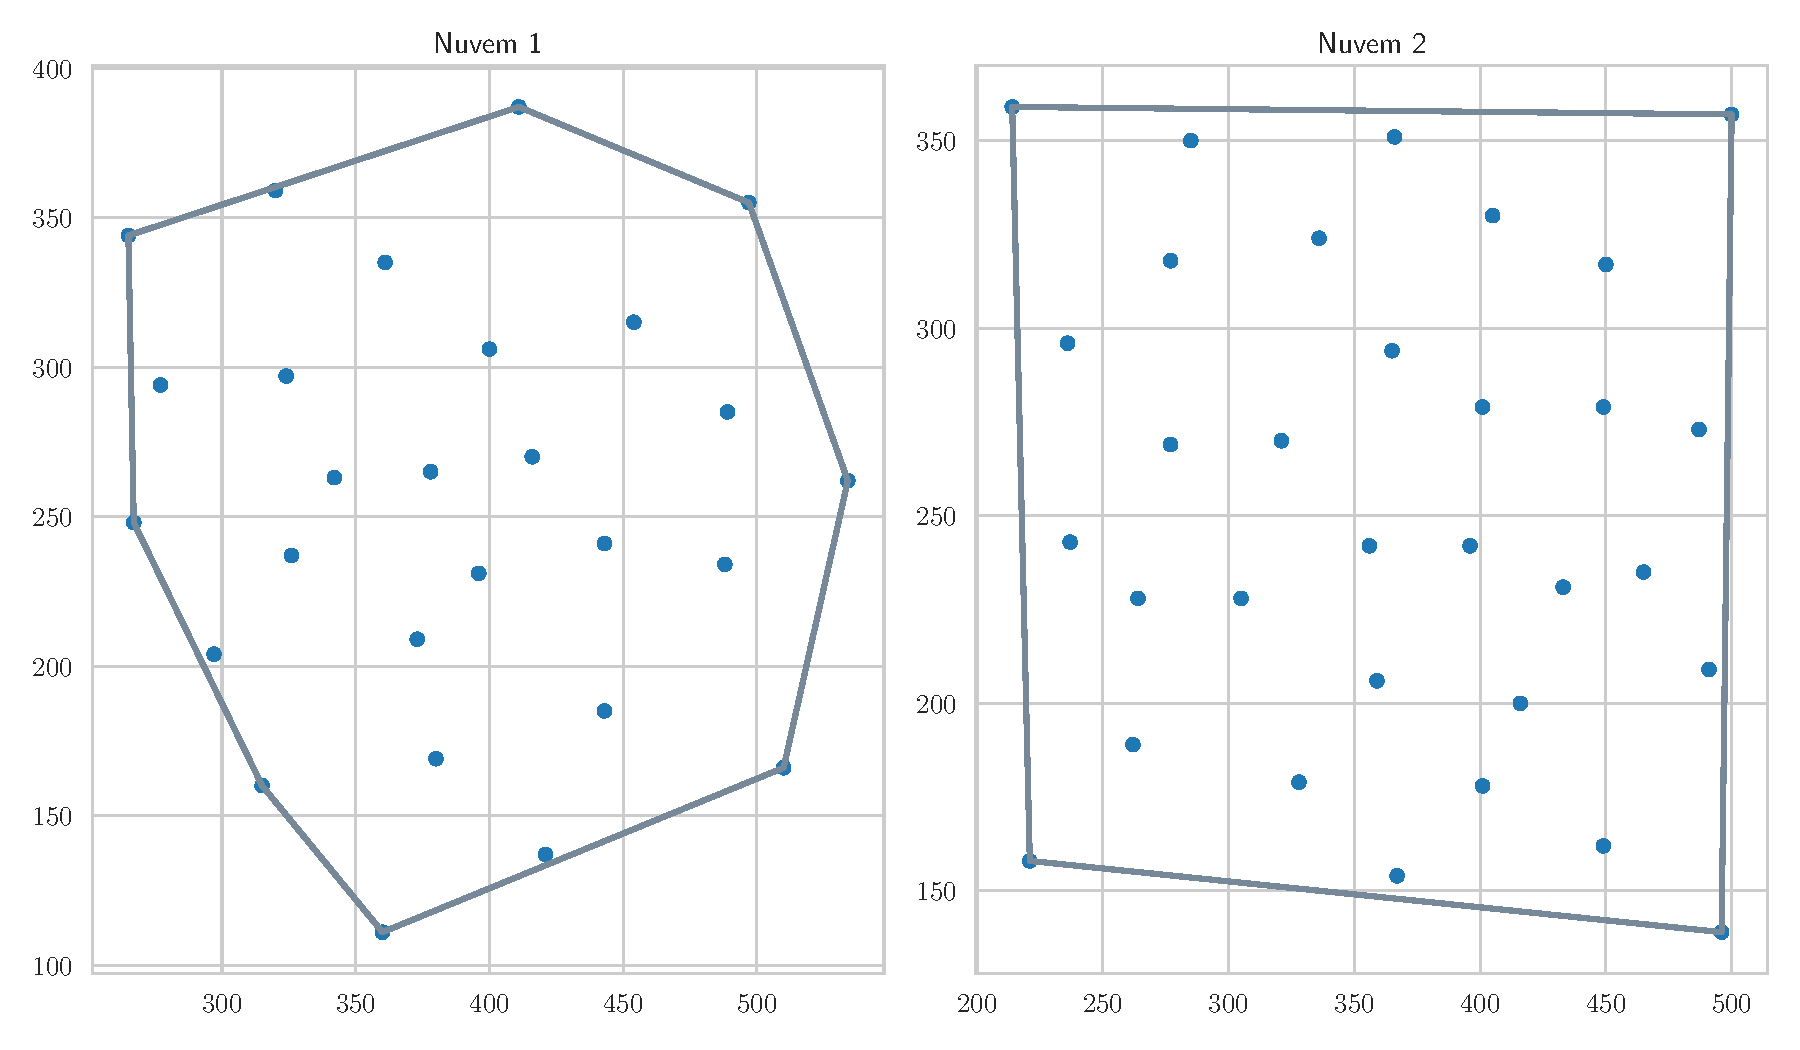
\includegraphics[scale=0.4]{nuvens.pdf}
  \caption{Nuvem1.txt e Nuvem2.txt}
  \label{fig:nuvens}  
\end{figure}

\subsection{Simulação de pontos aleatórios}

Além das nuvens de pontos definidas anteriormente como pontos de entrada, foi considerado um experimento no há geração aleatória de pontos. Cada subfigura em \ref{fig:aleatoria} possui 10.000 pontos aleatórios. 

\begin{figure}[H]
  \centering
  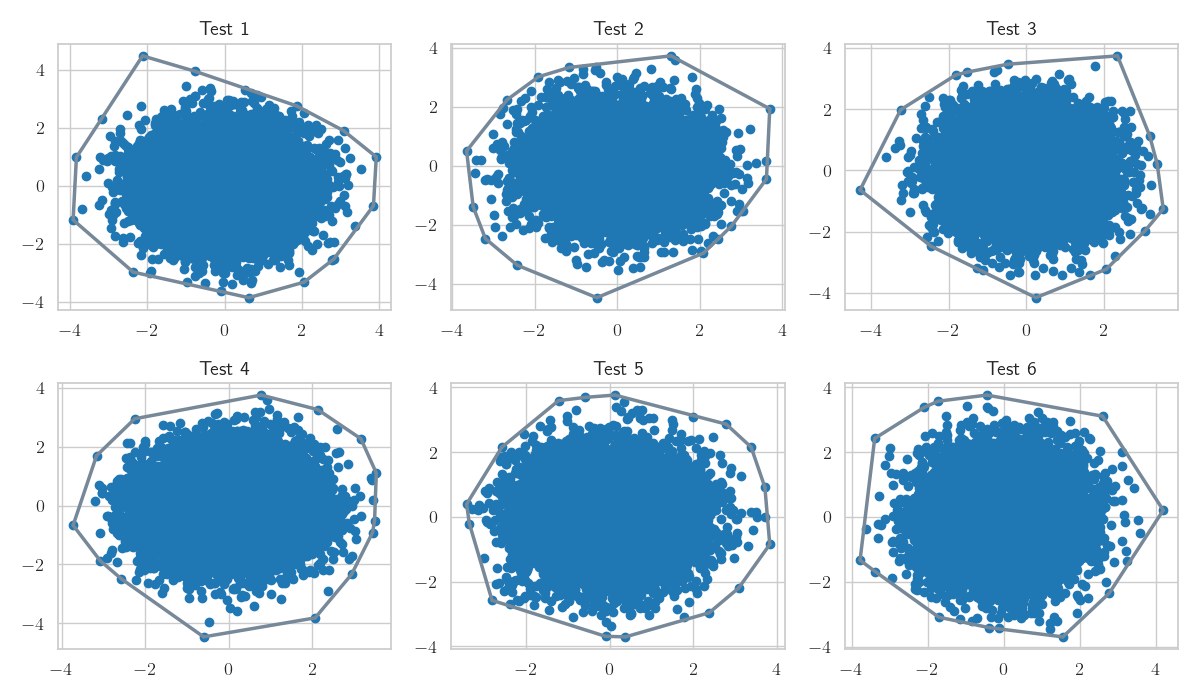
\includegraphics[scale=0.5]{random_test.png}
  \caption{Nuvem de pontos aleatórios}
  \label{fig:aleatoria}  
\end{figure}

Além disso podemos observar na Figura \ref{fig:aleatoria-runtime} o tempo de execução para diferentes tamanhos de entrada. Como esperado, temos que o tempo de execução é proporcional ao produto do tamanho da entrada vezes o número de pontos no fecho convexo.

\begin{figure}[H]
  \centering
  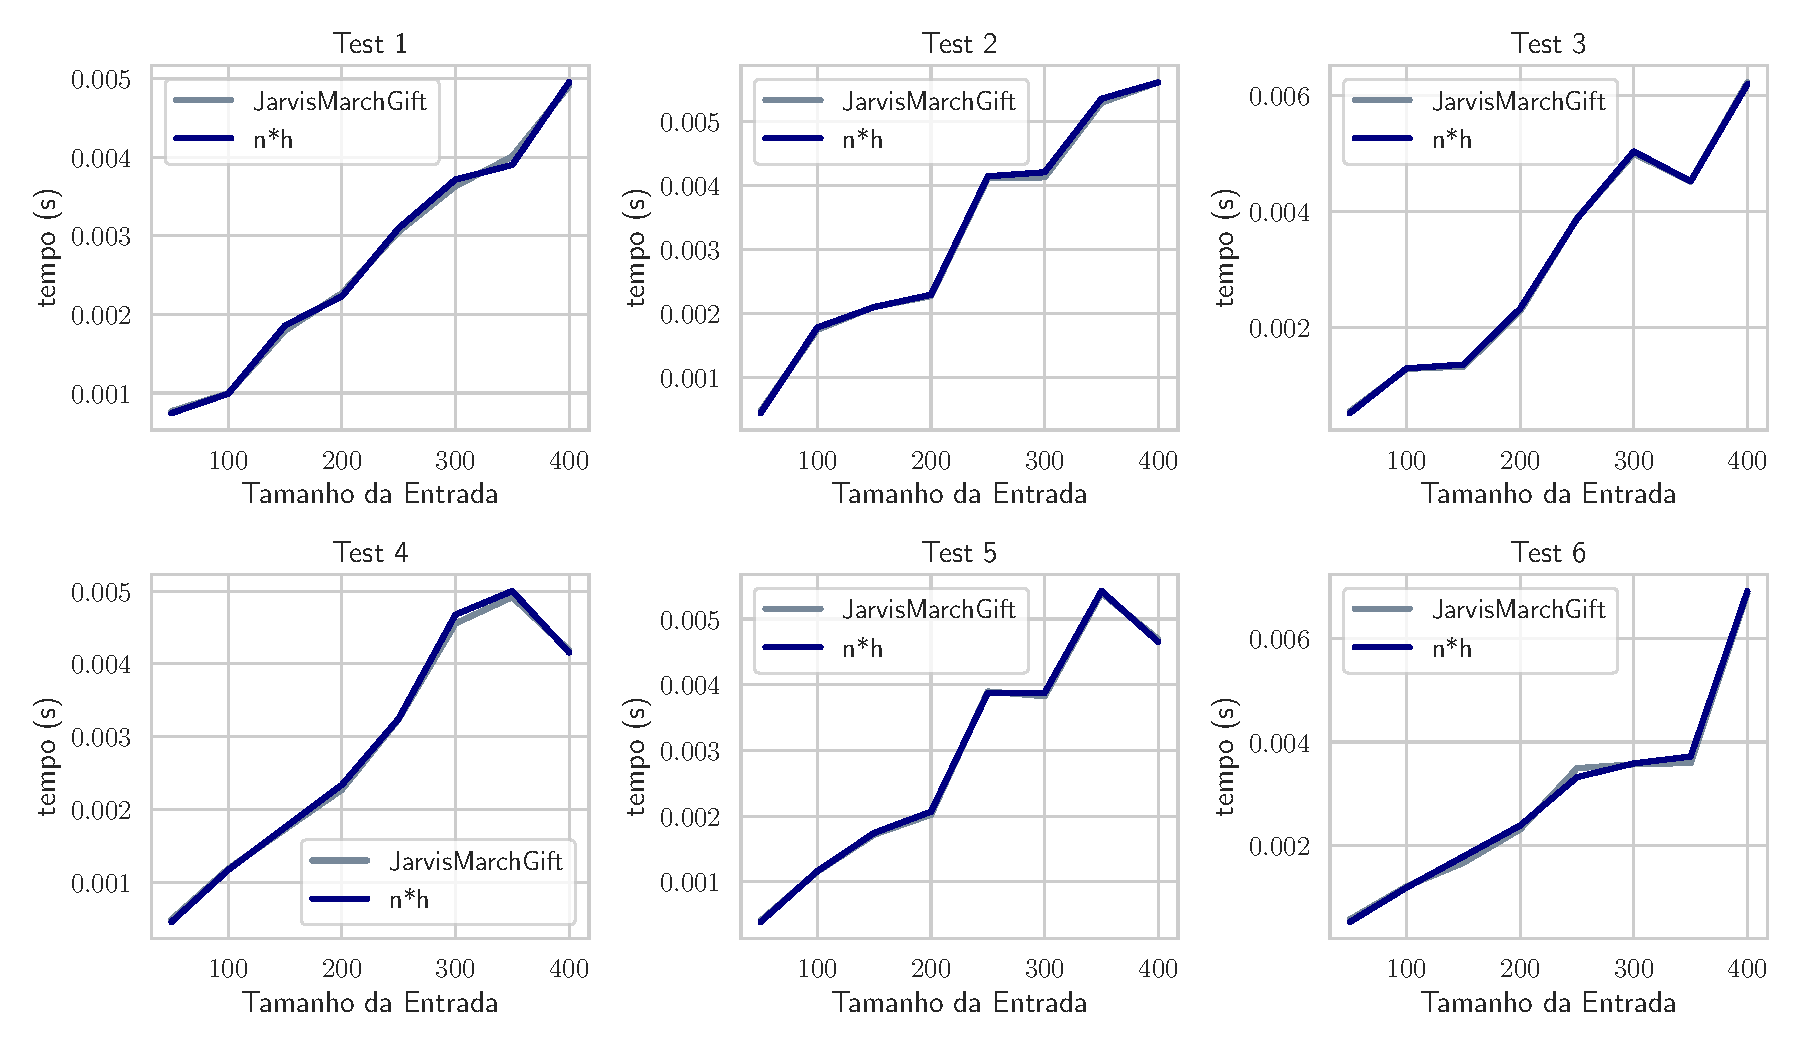
\includegraphics[scale=0.5]{runtime_test.pdf}
  \caption{Nuvem de pontos aleatórios}
  \label{fig:aleatoria-runtime}  
\end{figure}


\section{Conclusão}

Neste trabalho, foi apresentado o algoritmo Jarvis March, também conhecido como Gift Wrapping, para computar o fecho convexo de um conjunto de pontos. 

Além disso, foi realizado um experimento com a geração aleatória de pontos para avaliar o desempenho do algoritmo para diferentes tamanhos de entrada. Como esperado, o tempo de execução foi proporcional ao produto do tamanho da entrada vezes o número de pontos no fecho convexo.

Existem diversos algoritmos para computar o fecho convexo de um conjunto de pontos, e o algoritmo Gift Wrapping é um dos mais simples e eficientes. No entanto, a escolha do algoritmo mais adequado depende do contexto específico em que ele será aplicado.

\bibliographystyle{apa}
\bibliography{convex-hull/references.bib}

\end{document}